
\chapter{Хөгжүүлэлт}

Өөрийн тодорхойлсон шаардла, аргын дагуу хөгжүүлэлтийг хийхдээ дараах технологиудыг авч ашигласан.

\begin{itemize}
	\item OpenCV \cite{opencv} --- Анх 2000 онд танилцуулагдсан энэхүү нээлттэй эхийн сан нь өнөөдөр компьютерийн хараа\footnote{ Компьютерийн хараа (= Computer Vision)} -тай холбоотой ажил, судалгаануудад хамгийн өргөн ашиглагддаг бөгөө зураг боловсруулалтанд энэхүү сангийн санал болгосон функц, аргуудыг ашиглана
	\item Python \cite{python} --- OpenCV санг Python болон C++ хэл дээр ашиглах боломжтой байдаг бөгөөд зураг боловсруулах програм нь хөгжүүлэлтийн болон нийтэд нээлттэй тавих боломжийг үндэслэн Python хэлийг сонгон ашиглана
	\item PyPi\footnote{The Python Package Index (PyPI) --- \url{https://pypi.org/}} --- Зураг боловсруулж буй программаа энэхүү платформ дээр байршуулах ба хүссэн хэн нь ч Python багц удирдагч ашиглан амархан татан авах, ашиглах боломжтой болно
\end{itemize}

\section{Оролтын зураг боловсруулалт}

Оролтын зургаас үсэгт тэмдэгтүүдийг ялгахын тулд эхлээд зургаас шуугиан арилгах, гэрлийн нөлөөг багасгах, зургийг хоёртын болгон хувиргах гэх мэт урьдчилсан боловсруулалт хийсны үр дүнд хар цагаан зургаас ирмэг илрүүлэх боломжтой болдог.

John F. Canny -н ирмэг танилтын арга нь өөрөө зургаас шуугиан арилгах, гэрлийн нөлөөллийг багасгах, хар цагаан зураг болгон хувиргах зэрэг урьдчилсан боловсруулалтын аргуудыг ашигладаг бөгөөд дараах үе шатуудтай. Үүнд:

\begin{enumerate}
	\item Шуугиан арилгах --- Оролтын зургийн шуугиан нь ирмэг илрүүлэхэд шууд нөлөөлөх учир илрүүлэлтийн хамгийн эхний хэсэгт 5х5 хэмжээтэй Гаусс -н шүүлтүүрийг ашигладаг.
	\item Зургийн градиент олох --- Зургийн градиент гэдэг нь зургийн өнгө, пикселүүдийн идэвхжил нь чиглэлийн хувьд хэрхэн өөрчлөгдөж байгааг хэлдэг ба энэ хэсэгт Sobel kernel\footnote{\url{https://en.wikipedia.org/wiki/Sobel_operator}} ашиглан босоо, хэвтээ хоёр тэнхлэгийн градиентыг тооцоолдог.
	\item Non-maximum Suppression --- Өмнөх шатны гаралт дотроос ирмэг гэж үзэж буй пикселүүдийг дараагийн шатны боловсруулалтанд оруулах ба бусдыг нь 0 гэж тооцно. Цэгийн ирмэг эсэхийг тодорхойлохдоо зургийн градиент болон дотоод өндрийг (local maximum) тооцон мөн ирмэг, үгүй бол ирмэг гэж үзэхгүй.
	\item Hysteresis Thresholding --- Энэ хэсэг нь өмнөх шатны ирмэг гэж үзсэн цэгүүд дотор дахин хоёр утгаар зааглалт хийдэг. Өнгөний өөрчлөлттэй ирмэгийн цэгүүдийн утга дээд заагийн утгыг давж байвал баталгаатай ирмэг, харин доод заагийг давж чадахгүй цэгүүд ирмэг биш. Харин заагийн голд орших цэгүүд нь ямар нэг дээд зааг давсан цэгтэй холбоотой бол ирмэг, үгүй бол мөн ирмэг гэж тооцогдохгүй. Зураг \ref{fig:hysteresis}.
\end{enumerate}

\begin{figure}[H]
	\centering
	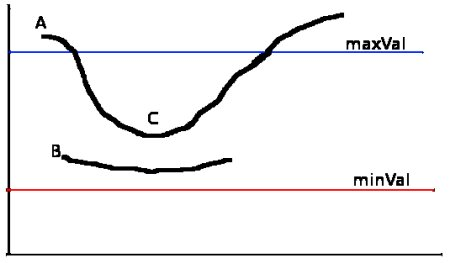
\includegraphics[width=0.6\linewidth]{images/hysteresis}
	\caption{Hysteresis Thresholding - \url{https://docs.opencv.org/trunk/da/d22/tutorial_py_canny.html} -аас зургийг авав.}
	\label{fig:hysteresis}
\end{figure}

Өөрөө хоёртын зураг болгож хувиргах -> шуугиан арилгах -> пикселүүдийг зааглах дарааллаар хар цагаан, зөвхөн цааш боловсруулалтанд чухал хэрэгтэй хэсгүүдийг оролтын зургаас ялгах нь John F. Canny -н ирмэг илрүүлэлтийн аргаас дутмаг болж байсан \ref{fig:sheet_final_edges} учир Canny -н ирмэг илрүүлэх аргыг сонгосон.

Үүний дараа ирмэг илрүүлсэн зургаас маягтын хамгийн чухал хэсэг болох бичвэрүүдийг хадгалж буй хүснэгтийг олох ёстой ба маягтын зургийг эгц дээрээс авч чадаагүй байх магадлалтай учир харах өнцгийн хувиргалтыг арилган, хүснэгтийг маягтын зурагнаас зүсэж авсан. Зураг \ref{fig:sheet_processing}.

Ингэхдээ хамгийн эхлээд оролтын зураг дээрээс contour буюу өнгө, идэвхжил ойролцоо хоорондоо холбоотой бүлэг муруйг \texttt{cv.findContours()} функцын тусламжтайгаар олж, олдсон контор цэгүүд дотроос хамгийн урт хүрээний урттай бүлэг буюу \ref{lst:biggest_contour} -аас булангийн дөрвөн цэгүүдийн вектор утгуудыг олсон. Зураг \ref{fig:sheet_final_contours}.

\begin{lstlisting}[caption={Хамгийн урт контор цэгүүд буюу энэ тохиолдолд бичвэр хадгалж буй хүснэгтийн ирмэг дээрх цэгүүд}, label={lst:biggest_contour}, language=Python]
biggest_contour = sorted(
	contours, 
	key=lambda contour: cv.arcLength(contour, True), 
	reverse=True
)[0]
\end{lstlisting}


\begin{figure}[H]
	\centering
	\begin{subfigure}{0.33\textwidth}
		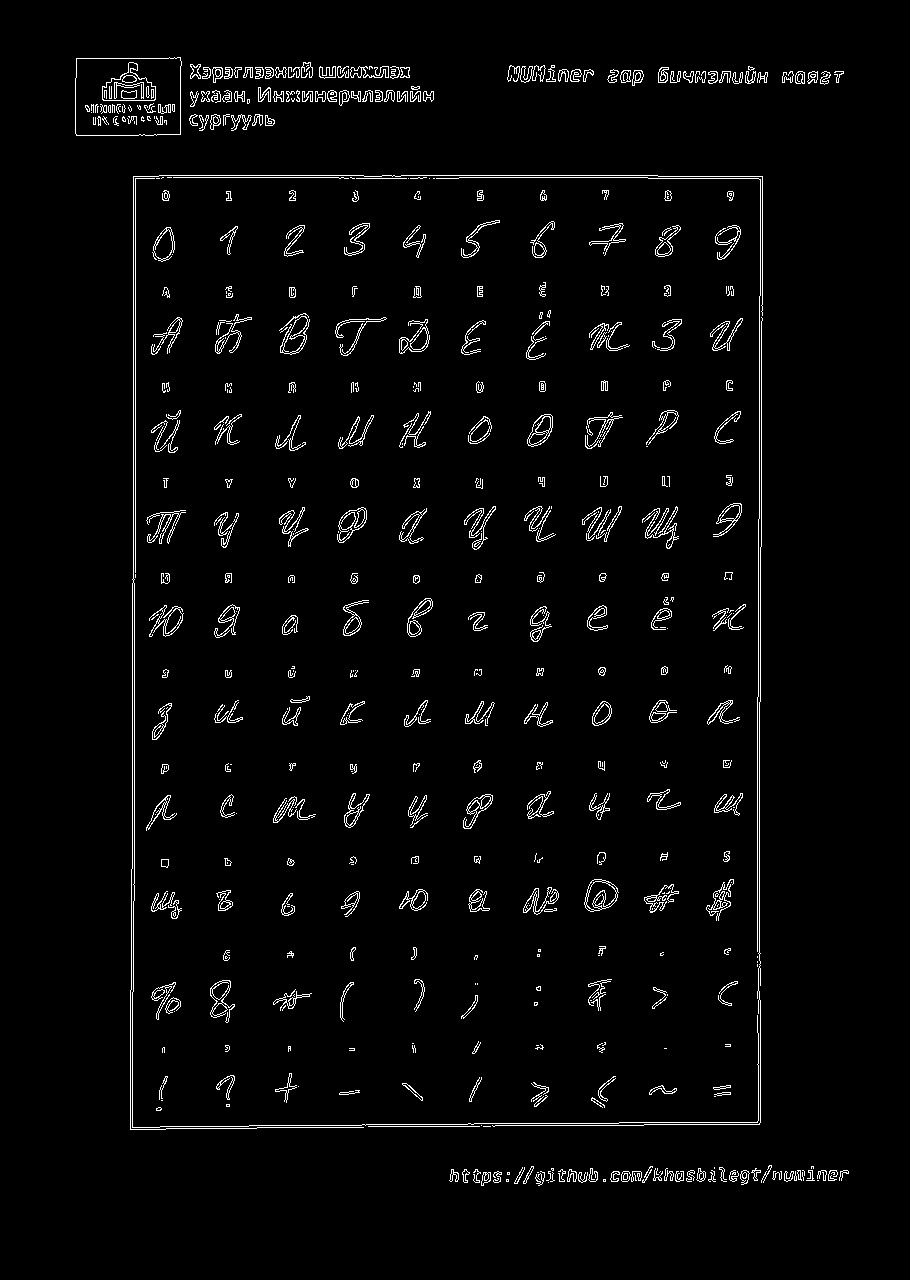
\includegraphics[width=0.9\linewidth]{images/sheet_final_edges}
		\caption{}
		\label{fig:sheet_final_edges}
	\end{subfigure}
	\begin{subfigure}{0.33\textwidth}
		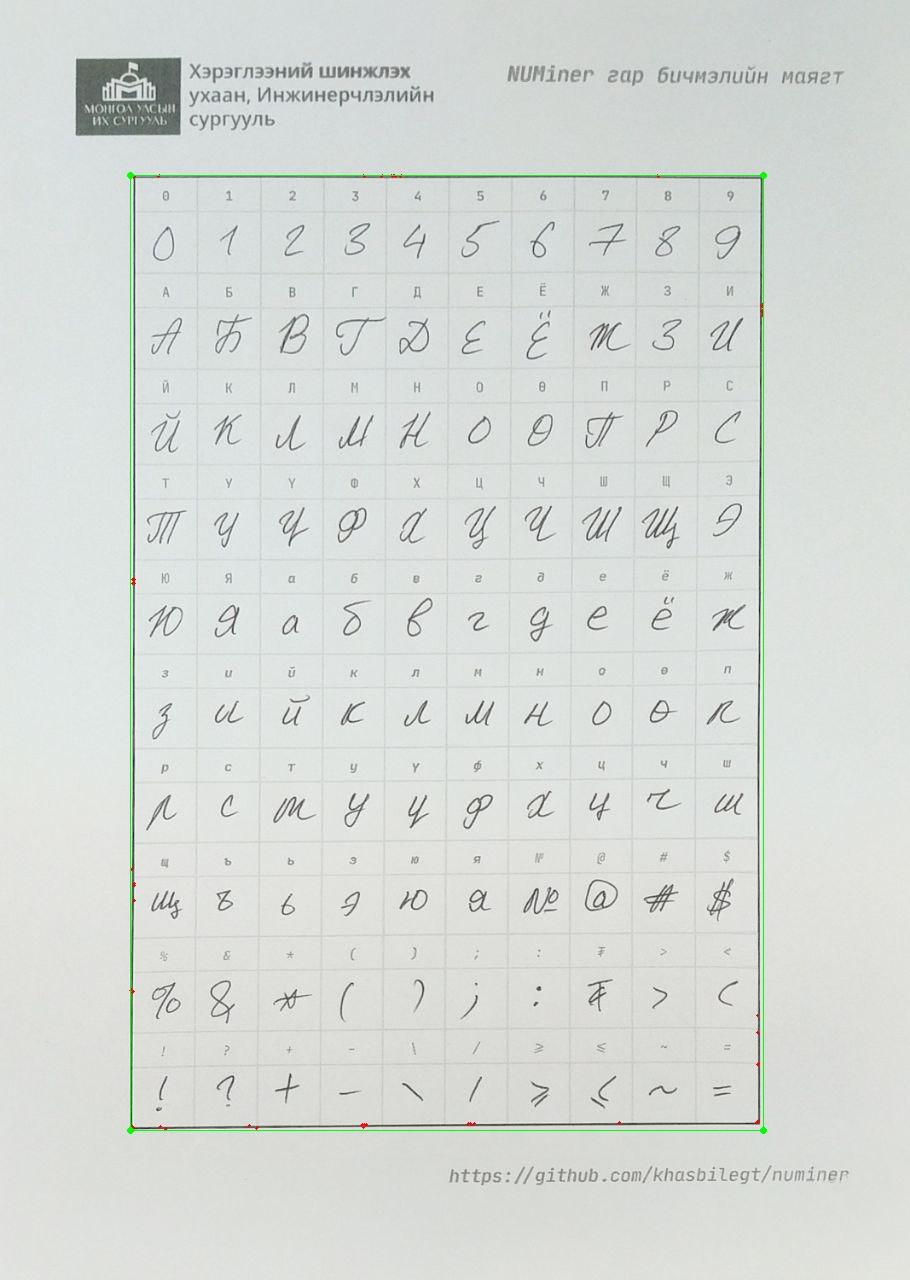
\includegraphics[width=0.9\linewidth]{images/sheet_final_contours}
		\caption{}
		\label{fig:sheet_final_contours}
	\end{subfigure}
	\begin{subfigure}{0.32\textwidth}
		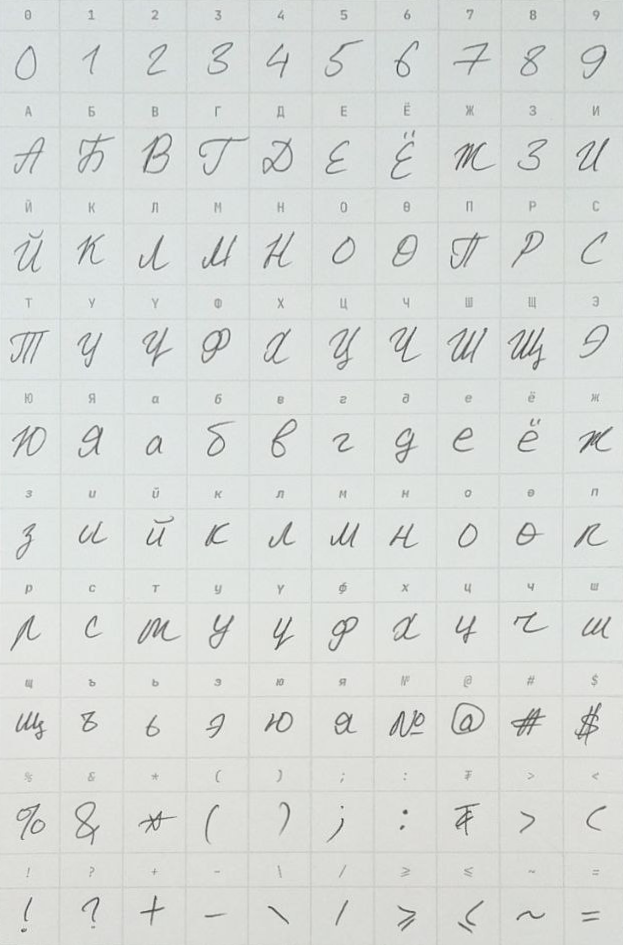
\includegraphics[width=0.85\linewidth]{images/sheet_final_transformed}
		\caption{}
		\label{fig:sheet_final_transformed}
	\end{subfigure}
	\caption{(a). Маягтын зураг дээр доод заагийг 100, дээд заагийг 200 утгаар Canny -н ирмэг илрүүлэх аргыг ашигласан үр дүн, (b). Илрүүлсэн ирмэгүүдээс контор цэгүүдийг олж, хамгийн урт хүрээний урттай контор цэгүүдийг багтаасан хамгийн жижиг тэгш өнцөгт олсон байдал, (c). Хамгийн том контор цэгүүдээс захын дөрвөн цэгийн утгуудыг олж харах өнцөгийн хувиргалтыг арилгасан байдал}
	\label{fig:sheet_processing}
\end{figure}

Код \ref{lst:biggest_contour} -н үр дүнд хүснэгтийн ирмэгүүд дээрх цэгүүдийн байршлыг олж авах бөгөөд эдгээрээс хамгийн захын дөрвөн цэг буюу яг зураг дээрх хүснэгтийн булангийн дөрвөн цэгийн байршлыг олох хэрэгтэй. Үүний тулд эхлээд \texttt{cv.approxPolyDP()} функцыг ашиглан \texttt{biggest\_contour} -н утгуудыг багасгасан. Энэхүү функц нь оролтын цэгүүд дотроос \texttt{epsilon} -д заасан утгаас бага зайнд орших цэгүүдийг тоймлон нэг шулуун болгодог функц юм. Хүснэгтийн булангийн дөрвөн цэгүүдийн олохын тулд \texttt{cv.approxPolyDP()} функцын үүсгэсэн цэгүүд бүрээс \texttt{x}, \texttt{y} -н утгуудын нийлбэр нь хамгийн их болон хамгийн бага утгуудыг олсон ба нийлбэр нь хамгийн бага байна гэдэг нь хүснэгтийн хамгийн зүүн дээд булангийн цэг, нийлбэр нь хамгийн их цэг нь хүснэгтийн хамгийн баруун доод цэг болно. Харин \texttt{x} - \texttt{y} буюу ялгавраар нь эрэмбэлсэн үед хамгийн их нь баруун дээд булангийн цэг, хамгийн бага нь зүүн доод булангийн цэг тус тус болно. Код \ref{extremePoints}.

\begin{lstlisting}[caption={Тоймлосон цэгүүдээс хүснэгтийн булангийн цэгүүдийг олох}, label=extremePoints, language=Python]
	points = tuple(
			(
					point[0][0] + point[0][1],
					point[0][0] - point[0][1],
					(point[0][0], point[0][1]),
			)
			for point in approx_curve
	)
	sum_sorted_points = sorted(
			points, key=lambda point: point[0]
	)
	diff_sorted_points = sorted(
			points, key=lambda point: point[1]
	)
	
	extreme_points = (
			sum_sorted_points[0][-1],
			diff_sorted_points[-1][-1],
			diff_sorted_points[0][-1],
			sum_sorted_points[-1][-1],
	)
	\end{lstlisting}

Маягт боловсруулалтын сүүлийн хэсэгт бичвэр агуулж буй хүснэгтийн булангийн дөрвөн цэгийн утгуудыг ашиглан харах өнцгийн хувиргалтыг (deskew) арилгах ёстой. Хэрэв оролтын зургийн эгц дээрээс нь авсан тэгш хувилбарыг $M_{original}$ гэж үзвэл ориг зургийг $M_{input} = A \cdot M_{original}$ гэж үзэж болно. Харин өнцгийн хувиргалтыг арилгахын тулд ориг зураг болох $M_{input}$ -г $A^{-1}$ буюу хувиргалтын функцын урвуугаар үржүүлбэл эгц, тэгш зураг $M_{original} = A \cdot A^{-1} \cdot M_{input}$ олох боломжтой. Гэвч эндээс мэдэгдэж байгаа нь оролтын зураг дээрх хүснэгтийн цэгүүд болон эгц дээрээс нь авсан үед хаана байх ёстой цэгүүд бөгөөд OpenCV -н \texttt{cv.findHomography()} функц нь параметртаа авах хоёр цэгийн хувиргалтын матрицыг олдог. Үүнийг ашиглан оролтын зургийн харах өнцгийн хувиргалтыг арилган (Код \ref{lst:deskew}) дараагийн шатанд тэмдэгтүүдийг ялгахад бэлэн болж байгаа юм. Зураг \ref{fig:sheet_final_transformed}.

\begin{lstlisting}[caption={Харах өнцгийн хувиргалтыг арилгах}, label={lst:deskew}, language=Python]
homog, _ = cv.findHomography(
	np.array(extreme_points),
	np.array(bounding_rect_points),
)
transformed = cv.warpPerspective(
	source,
	homog,
	(int(source.shape[1]), int(source.shape[0])),
)
\end{lstlisting}

\section{Тэмдэгтүүдийг хүснэгтээс салгах}

Оролтын зураг боловсруулагдаж дуусаад дан бичвэр агуулсан хүснэгтийг илрүүлсэний дараа хүснэгтийн мөр, баганы тоогоор нүд болгоныг ялган авсан ба ингэхдээ гараар бөглөх хэсгийн дээд талын тэмдэгтийн нэрүүд (label) агуулсан хэсгүүдийг оруулахгүй байхаар гүйцэтгэсэн. Зураг \ref{fig:sheet_final_segmented}.

\begin{figure}[H]
	\centering
	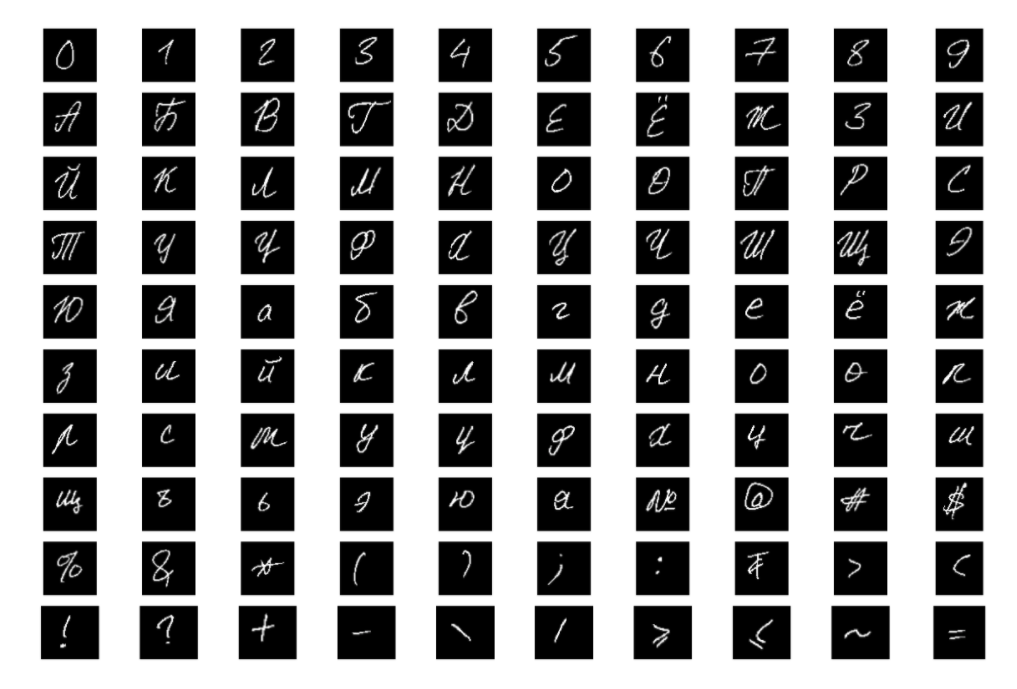
\includegraphics[width=1\linewidth]{images/sheet_final_segmented}
	\caption{Оролтын зураг боловсруулалтын үр дүнгээс гараар бичигдсэн тэмдэгтүүдийг нэг нэгээр нь ялган авсан байдал}
	\label{fig:sheet_final_segmented}
\end{figure}

\textit{Шаардлага №\ref{criteria:3}} -т нийцүүлэх зорилгоор маягт доторх тэмдэгтүүд өөрчлөгдөх эсвэл маяг тэр чигтээ өөрчлөгдөх тохиолдолд хүснэгтийн бүх нүдийг дүүргэх шаардлагагүй ба оролтын маягтыг өгөхдөө тодорхойлох тэмдэгтүүдийн дараалалд \texttt{skip\_char} байгаа эсэхийг шалгаж хэрэв байгаа бол тэр тэмдэгттэй харгалзах нүдийг боловсруулалтанд хэрэгсэхгүй. Үүний жишээг Зураг \ref{fig:sheet_1} -аас харж болох ба маягтын тэмдэгтүүдийн дараалал (\texttt{label\_seq}) Код \ref{lst:sheet_1_label_seq} болно. \texttt{skip\_char = "*"} тухайн тэмдэгттэй харгалзах нүдийг гаралтанд тооцохгүй.

\begin{lstlisting}[caption={Хамгийн эхний маягтын хувилбарын нүднүүд, тэдгээрт харгалзах тэмдэгтүүдийн дараалал}, label={lst:sheet_1_label_seq}, language=Python]
labelSeq = ('0', '1', '2', '3', '4', '5', '6', '7', '8', '9', 
					  '№', '₮', '*', '*', '*', '*', '*', '*', '*', '*', 
					  'А', 'Б', 'В', 'Г', 'Д', 'Е', 'Ё', 'Ж', 'З', 'И', 
					  'Й', 'К', 'Л', 'М', 'Н', 'О', 'Ө', 'П', 'Р', 'С', 
					  'Т', 'У', 'Ү', 'Ф', 'Х', 'Ц', 'Ч', 'Ш', 'Щ', 'Э', 
					  'Ю', 'Я', '*', '*', '*', '*', '*', '*', '*', '*', 
					  'а', 'б', 'в', 'г', 'д', 'е', 'ё', 'ж', 'з', 'и', 
					  'й', 'к', 'л', 'м', 'н', 'о', 'ө', 'п', 'р', 'с',
					  'т', 'у', 'ү', 'ф', 'х', 'ц', 'ч', 'ш', 'щ', 'ъ', 
					  'ы', 'ь', 'э', 'ю', 'я', '*', '*', '*', '*', '*')
\end{lstlisting}

\section{Гаралт}

Хүснэгтээс ялган авсан зураг бүр дээр дахин боловсруулалт хийх ба үр дүнд хоёртын (binary), 28х28 хэмжээтэй зураг үүсэх ёстой. Энэ шатны оролтын зураг нь хүснэгтээс ялган авсан нэг тэмдэгтийн зураг байх бөгөөд тэдгээр зургууд гаралтын зургийн байх ёстой хэмжээнээс хамаагүй том, дээр нь харьцаанууд нь харилцан адилгүй байх магадлалтай.

Эхний алхамд гар бичмэлийг бөглөсөн хүн тэмдэгтүүдийг тухайн нүдний аль нэг хэсэгт маш жижиг хэмжээтэйгээр эсвэл хангалттай дүүргэж ямар ч байдлаар бичиж болох учраас оролтын зургийг шууд гаралтын зургийн хэмжээнд тааруулан хэмжээг нь багасгаж болохгүй. Тийм учраас оролтын зураг дээр дахин тоон дүрс боловсруулалт хийх ёстой. Оролтын зурагт тэмдэгттэй ямар ч холбоогүй ямар нэг пиксел, шуугиан байх магадлалтай учир 5х5 хэмжээтэй \texttt{cv.GaussianBlur()} ашигласан ба \texttt{cv.adaptiveThreshold()} -аар пикселүүдийг зааглан хоёртын зургийг гарган авсан. \ref{fig:letter_a_binary} Оролтын зургийн пикселийн утгууд бүдэг, тод ямар ч байх боломжтой учир заагийн утга нь оролтоос хамааран динамик байдлаар тодорхойлогддог байх ёстой.


\begin{figure}[H]
	\centering
	\begin{subfigure}{0.24\textwidth}
		
\includegraphics[width=0.9\linewidth]{images/letter_a_binary}
		\caption{63х63}
		\label{fig:letter_a_binary}
	\end{subfigure}
	\begin{subfigure}{0.24\textwidth}
		
\includegraphics[width=0.9\linewidth]{images/letter_a_cropped}
		\caption{41х41}
		\label{fig:letter_a_cropped}
	\end{subfigure}
	\begin{subfigure}{0.24\textwidth}
		
\includegraphics[width=0.9\linewidth]{images/letter_a_resized}
		\caption{28x28}
		\label{fig:letter_a_resized}
	\end{subfigure}
	\begin{subfigure}{0.24\textwidth}
		
\includegraphics[width=0.9\linewidth]{images/letter_a_final}
		\caption{28х28}
		\label{fig:letter_a_final}
	\end{subfigure}

	\caption{(a). Хүснэгтээс салган авсан А үсэг, (b). Зургаас контор цэгүүдийг олж бүгдийг нь багтаах хамгийн жижиг тэгш өнцөгт олж харьцааг нь алдагдуулалгүйгээр талуудыг тэнцүүлсэн байдал, (c). Талыг нь тэнцүүлсэн зургийг 28х28 болгож багасгасан байдал, (d). Зурагны пикселүүдийг Otsu -н зааглалтын аргыг ашиглан хоёртын зураг болгон хувиргасан ба гаралтанд бэлэн болсон зураг}
	\label{fig:letter_a}
\end{figure}

Урьдчилсан боловсруулалт хийгдсэн зургаас онцлог шинжүүдийг задлан авах (Feature extraction) буюу энэ тохиолдолд хүний гараар бөглөсөн тэмдэгтийн хэсгийг оролтын зургаас илрүүлэх хэрэгтэй. Үүний тулд мөн \texttt{cv.findContours()} функцыг ашигласан ба хүснэгтийн контор цэгүүд дээр боловсруулалт хийж байснаас ялгаатай нь тэмдэгтээс олдсон бүх контор цэгүүдийг багтаасан хамгийн жижиг тэгш өнцөгт (bounding rectangle) -г олж тооцоолж зөвхөн тэр хэсгийг зургаас тасдан авна. Код \ref{lst:letter_crop}.

\begin{lstlisting}[caption={Тэмдэгтээс контор цэгүүдийг олж бүгдийг нь багтаасан хамгийн жижиг тэгш өнцөгтөөр тасдан авах}, label={lst:letter_crop}, language=Python]
contours, _ = cv.findContours(
		binary, cv.RETR_EXTERNAL, cv.CHAIN_APPROX_SIMPLE
)
sorted_contours = sorted(
		contours,
		key=lambda ctr: cv.contourArea(ctr),
		reverse=True,
)

point_x = []
point_y = []

for x, y, w, h in (
		cv.boundingRect(ctr) for ctr in sorted_contours
):
		point_x.append(x)
		point_x.append(x + w)
		point_y.append(y + h)
		point_y.append(y)

points = list(zip(sorted(point_x), sorted(point_y)))

max_col = points[-1][0] # Хэвтээ тэнхлэгийн хамгийн дээд утга
max_row = points[-1][1] # Босоо  тэнхлэгийн хамгийн доод утга
min_col = points[0][0] # Хэвтээ тэнхлэгийн хамгийн доод утга
min_row = points[0][1] # Босоо тэнхлэгийн хамгийн дээд утга

w_a = max_col - min_col
h_a = max_row - min_row

if w_a > h_a:
		diff_x = 0
		diff_y = (w_a - h_a) // 2
elif w_a < h_a:
		diff_x = (h_a - w_a) // 2
		diff_y = 0
else:
		diff_x = 0
		diff_y = 0

diff_x += cls._BORDER_THICKNESS # _BORDER_THICKNESS: 2
diff_y += cls._BORDER_THICKNESS # _BORDER_THICKNESS: 2

cropped = binary[min_row:max_row, min_col:max_col]
cropped = cv.copyMakeBorder(
		cropped,
		diff_y,
		diff_y,
		diff_x,
		diff_x,
		borderType=cv.BORDER_CONSTANT,
		value=[0, 0, 0],
)
\end{lstlisting}

Үүссэн тэгш өнцөгтийн хэмжээ нь гараар бичигдсэн тэмдэгтээс хамааран ямар ч байж болох учир зургийг гаралтын хэмжээтэй болгож жижигрүүлэхээс өмнө талуудыг адил буюу, тэгш дөрвөлжин зураг болгон хувиргах шаардлагатай. Үүнээс гадна EMNIST -н зураг боловсруулалтын үйл явцад үндсэн тэмдэгтийн зургийн талуудыг харьцааг нь алдагдуулалгүйгээр адилхан болгосны дараа тэмдэгтийг ирмэгт наалдуулахгүйн тулд 2 пиксел хүрээ нэмж өгч байсныг (Зураг \ref{fig:emnist-conversion}) давхар гүйцэтгэснийг Код \ref{lst:letter_crop} -оос мөн харж болно. Зураг \ref{fig:letter_a_cropped}.

Ингээд талуудыг нь адилтгасан мөн 2 пиксел хүрээ нэмсэн зургаа \texttt{cv.resize()} функц ашиглан жижигрүүлж үүссэн зурагт дахин thresholding хийснээр гаралтын зураг (Зураг \ref{fig:letter_a_final}) боловсруулагдаж дуусах ба нэг тэмдэгтийн зургийн боловсруулалт хэрхэн хийгдсэнийг Хавсралт \ref{appendix:get_char} -ээс үзнэ үү.